\documentclass[11pt]{aghdpl}
\usepackage[polish]{babel}
\usepackage[utf8]{inputenc}
\usepackage{enumitem}
\usepackage{listings}
\usepackage{graphicx}

\author{Wojciech Kasperek, Krzysztof Spytkowski, Izabela Śmietana}
\shortauthor{W. Kasperek, K. Spytkowski, I. Śmietana}

\titlePL{Problem istnienia k-kliki}
\titleEN{}

\shorttitlePL{Problem istnienia k-kliki}
\shorttitleEN{}

\thesistype{Projekt zaliczeniowy:}

\supervisor{dr Adam Sędziwy}

\degreeprogramme{Informatyka}

\subject{Badania operacyjne i teoria złożoności obliczeniowej}

\date{2014}

\department{Katedra Informatyki Stosowanej}

\faculty{Wydział Elektrotechniki, Automatyki,\protect\\[-1mm] Informatyki i Inżynierii Biomedycznej}

%---------------------------------------------------------------------------

\begin{document}

\titlepages
\vspace*{-20mm}
\tableofcontents
\clearpage

\chapter{Zarys problemu}
\label{cha:zarys}

Wybrany przez nas temat dotyczy kliki, dlatego omówienie zaczniemy od~wprowadzenia tego pojęcia. 
Kliką w~grafie nazywamy zbiór wierzchołków, w~którym każda para wierzchołków jest połączona krawędzią, 
czyli podgraf będący grafem pełnym. Problem istnienia k-kliki polega na~stwierdzeniu 
czy~w~danym grafie istnieje klika o~podanym rozmiarze $k$. Problem ten należy do~klasy NP, co~oznacza, że~rozwiązanie 
można zweryfikować w czasie wielomianowym (mając podane wierzchołki należące do~szukanej
kliki możemy w~czasie $O(k^2)$ sprawdzić, czy faktycznie jest to klika).

Problem istnienia k-kliki jest także jednym z~pierwszych zidentyfikowanych problemów NP-zupełnych. 
Problem NP-zupełny to~problem, który należy do klasy NP oraz dowolny problem należący do~NP może być do~niego 
zredukowany w~czasie wielomianowym. NP-zupełność naszego problemu wynika z~NP-zupełności problemu 
zbioru niezależnego. Problem ten to~pytanie czy~dla danego grafu $G$ i~liczby $k$, istnieje w~$G$ zbiór 
niezależny (zbiór wierzchołków niepołączonych żadnymi krawędziami) o~$k$~wierzchołkach. W~naszym problemie 
w~grafie istnieje klika o~rozmiarze $k$~wtedy i~tylko wtedy gdy~w~dopełnieniu grafu istnieje zbiór niezależny 
o~rozmiarze $k$.

Ze~względu na~klasę złożoności problemu i~brak odpowiednio szybkich algorytmów dokładnych, w~naszym projekcie 
posłużymy się~algorytmem przybliżonym (genetycznym). 

\section{Klasyczny algorytm genetyczny}
\label{sec:algGenetyczne}
Postawiony problem definiuje środowisko, w~którym istnieje pewna populacja osobników. Każdy z~osobników ma~
przypisany pewien zbiór informacji stanowiących jego genotyp, a~będących podstawą do~utworzenia
fenotypu. Fenotyp to~zbiór cech podlegających ocenie (przez funkcję przystosowania).
Innymi słowy - genotyp opisuje proponowane rozwiązanie problemu, a~funkcja przystosowania ocenia, jak
dobre jest to~rozwiązanie.

Genotyp składa się~z~chromosomów, w~których zakodowany jest fenotyp i~ewentualnie pewne informacje
pomocnicze dla~algorytmu genetycznego. Chromosomy składają się~z~genów.

Klasyczny algorytm genetyczny składa się~z~następujących kroków:
\begin{enumerate}[noitemsep]
\item inicjalizacja – utworzenie populacji początkowej, wybór ustalonej liczby osobników i~nadanie wartości losowych 
genom wchodzącym w~skład ich~chromosomów;
\item ocena przystosowania – obliczenie wartości funkcji przystosowania dla~każdego osobnika;
\item selekcja – wybór osobników, które będą brać udział w~tworzeniu nowej populacji;
\item zastosowanie operatorów genetycznych – na~grupie osobników wybranych drogą selekcji działają
operatory genetyczne (krzyżowanie i~mutacja);
\item utworzenie nowej populacji – osobniki otrzymane jako rezultat działania operatorów
genetycznych wchodzą w~skład nowej populacji. Cała poprzednia populacja jest~zastępowana przez
tak~samo liczną nową populację potomków;
\item sprawdzenie warunku stopu algorytmu - wyprowadzenie ''najlepszego'' osobnika (o~największej wartości funkcji 
przystosowania). Jeżeli osobnik ten~spełnia postawione w~zadaniu warunki to~algorytm kończy pracę, w~przeciwnym 
razie przechodzi do~punktu 2~(działając już na populacji potomków).

\end{enumerate}
\section{Własna interpretacja problemu i adaptacja algorytmu}
\label{sec:podejscie}
Zaimplementowany przez nas~sposób rozwiązania problemu jest oparty na~powyższym algorytmie, jednak program 
udostępnia wiele możliwości dostosowywania go. Dzięki temu możemy badać skuteczność poszczególnych metod 
w~odniesieniu do~zadanego problemu i~ustalanych przez~użytkownika parametrów wejściowych.

W~aplikacji zawarte zostały dwa sposoby kodowania osobnika, binarny i~grupowy. Są~to~zupełnie różne sposoby
zapisu informacji w~chromosomie, przez~co~przebieg działania algorytmu jest odmienny dla każdego z~tych kodowań. Mimo różnic w~genotypach, 
w~obu przypadkach fenotypem jest graf.
Program udostępnia również trzy różne sposoby selekcji możliwe do~zastosowania w~problemie istnienia k-kliki oraz~rozmaite 
typy krzyżowań. Opisy wszystkich kodowań, operatorów genetycznych, funkcji oceny oraz motywacja wyboru właśnie takich, 
znajdują się~w~dalszych rozdziałach.

\chapter{Kodowanie i funkcja przystosowania}
\label{cha:encoding}
W~obu kodowaniach chromosomem jest tablica (o~wielkości odpowiadającej liczbie wierzchołków w~grafie), której 
indeksy oznaczają kolejne wierzchołki zadanego grafu.
\section{Binarne}
\label{sec:binary}
W binarnym kodowaniu chromosomu zasada jest~następująca: gen ''0'' w~chromosomie oznacza przynależność danego wierzchołka 
do~podgrafu, ''1'' oznacza, że~tego~wierzchołka nie~ma~w~podgrafie.
\section{Grupowe}
\label{sec:group}
Kodowanie grupowe, w~odróżnieniu od~binarnego, dopuszcza przyjmowanie przez geny więcej niż~dwóch wartości - możliwych 
jest ich~tyle, ile~aktualnie wynosi liczba grup. Każda grupa - a~więc~każda wartość $\langle0; n)$, gdzie $n$~to~liczba grup - odpowiada 
podgrafowi w~zadanym grafie. Takie podejście pozwala zawrzeć w~genotypie znacznie więcej informacji, ponieważ każdy podgraf jest potencjalnym 
rozwiązaniem. 

Ocena osobnika w~tym wypadku polega na~ocenie osobno każdej grupy i~wyłonieniu najlepszej z~nich. Wartość przystosowania tej~grupy odpowiada przystosowaniu 
całego osobnika.

Ważnym aspektem jest odpowiednie numerowanie poszczególnych grup. Po~każdej ocenie następuje przepisanie numeracji tak, aby~najmniejszy
numer odpowiadał najlepszemu podgrafowi, a~odpowiednio większe kolejnym. Ma~to~bardzo duże znaczenie przy~operacji krzyżowania, gdzie chroni nas 
przed utratą najlepiej ocenionych rozwiązań. Dla~przykładu, ten~sam dobrze przystosowany zbiór wierzchołków w~różnych chromosomach mógł
należeć do~grup o~różnych numerach, przez~co~nowo powstały w~wyniku krzyżowania osobnik otrzymywał informacje o wspomnianym podgrafie rozbite
na~dwie grupy (czyli je~tracił).

Ostatnim ważnym elementem dotyczącym omawianego kodowania jest liczba grup. W~populacji cały czas utrzymywana jest taka sama ilość 
grup u~każdego osobnika, jednak, w~wybranych iteracjach, liczba grup dla całej populacji jest zmniejszana, za~każdym razem o jeden. 
Likwidowany, najsłabiej przystosowany podgraf, zostaje dołączany do~drugiego aktualnie najsłabszego.

Częstość usuwania grup zależy od~zadanej ilości iteracji, tak, że~w~końcowych iteracjach pozostają jedynie dwie grupy.

\section{Funkcja przystosowania}
\label{sec:fitnessFunction}
W obu powyższych kodowaniach zastosowanliśmy tę~samą funkcje przystosowania. Wzór pozwalający
obliczyć przystosowanie $j$-tego osobnika w populacji (oznaczanego jako $x_j$) to:           

$$
f(x_j) = \smash{\displaystyle\max_{0 \leq i \leq n-1}} \left(\frac{e_{j_i}}{\frac{v_{j_i}(v_{j_i} - 1)}{2}}\frac{k - |v_{j_i} - k|}{k}\right) 
$$

gdzie $n$ oznacza liczbę grup wierzchołków w~chromosomie, $i$ identyfikuje kolejną grupę 
(dla~kodowania binarnego rozpatrujemy tylko $i~=~0$), $e_{j_i}$~i~$v_{j_i}$~to~odpowiednio liczba krawędzi i wierzchołkół $i$-tego podgrafu, a~$k$~jest
rozmiarem szukanej kliki.

Pierwszy ułamek wyraża ''gęstość'' grafu, czyli stosunek liczby jego krawędzi do~pożądanej wartości (liczby krawędzi w~k-klice); natomiast
drugi to~kara dotycząca rozmiaru ocenianego grafu (przyjmuje wartość $1$~tylko i~wyłącznie wtedy gdy~rozmiary są~równe).

\chapter{Selekcja}
\label{cha:selection}
Selekcja dokonuje wyboru osobników będących rodzicami dla~nowego pokolenia.
W~zależności od~wartości funkcji przystosowania danego osobnika w~populacji ma~on~większe (gdy jest ''dobry'') lub~mniejsze 
(gdy jest ''słaby'') szanse na~znalezienie się~w~kolejnym pokoleniu. 
\section{Turniejowa}
\label{sec:tournament}
Polega na~podziale populacji na~grupy n-osobników (w~naszej implementacji są~to~grupy 3-osobnikowe). Z~każdej 
z~tych grup wybierany jest najlepiej przystosowany osobnik, który zostaje dołączony do~grona rodziców.

\section{Koła ruletki}
\label{sec:roulette}
Polega na~n~krotnym ($n$ - liczba osobników w populacji) losowaniu osobników ze~starej populacji i~przepisaniu ich do~grupy rodziców,
przy czym osobniki w~tej~grupie mogą się~powtarzać. Przed rozpoczęciem losowania każdemu $j$-temu osobnikowi nadawane jest prawdopodobieństwo wylosowania, 
które wyliczane jest zgodnie ze~wzorem:
$$
P(x_j) = \frac{f(x_j)}{\sum\limits_{i=1}^n{f(x_i)}}
$$
gdzie $f$~jest funkcją oceny, a~$x$~to~osobniki populacji.
 
\section{Rankingu liniowego}
\label{sec:linear}
Selekcja ta jest bardzo podobna do~metody koła ruletki. Modyfikacja polega jedynie na~zmianie funkcji 
określającej prawdopodobieństwo wyboru danego osobnika. Przed przystąpieniem do~tej~selekcji należy nadać każdemu z~osobników 
pewną wartość (pozycje w~rankingu) zależną od~jego położenia na~liście posortowanej względem wartości funkcji 
przystosowania. Wzór pozwalający obliczyć prawdopodobieństwo wyboru $j$-tego osobnika to:
$$
P(x_j) = \frac{pos(x_j)}{\sum\limits_{i=1}^n{f(x_i)}}
$$
gdzie $f$~to~funkcja oceny, $pos$ to~funkcja zwracająca położenie na~posortowanej liście, a~$x$~to~osobniki populacji.

\chapter{Krzyżowanie}
\label{cha:crossing}
Zadaniem krzyżowania jest wymiana ''materiału genetycznego'' pomiędzy dwoma osobnikami w~populacji. Polega na~połączeniu 
niektórych (wybranych od~rodziców) genów w~jeden nowy genotyp (lub w~dwa, jeśli w~wyniku krzyżowania powstaje dwóch potomków). Kojarzenie ma~sprawić, że~potomek dwóch osobników rodzicielskich 
ma~zespół cech, który jest kombinacją ich~cech (może się~zdarzyć, że~tych najlepszych).

\section{Jednopunktowe z dwoma potomkami}
\label{sec:jedenDwa}
Polega na podziale dwóch chromosomów (pochodzących od~rodziców) na~dwie części (niekoniecznie równe) i~utworzeniu z~nich 
dwójki dzieci: pierwsze dziecko składa się~z~początkowej części materiału genetycznego pierwszego rodzica i~końcówki drugiego, 
natomiast drugie dziecko otrzymuje początek materiału genetycznego drugiego rodzica i~końcówkę pierwszego.

\section{Jednopunktowe z jednym potomkiem}
\label{sec:jedenJeden}
Krzyżowanie analogiczne do~powyższego, ale~w~wyniku powstaje jedno dziecko, końcówka materiału genetycznego pierwszego 
rodzica i~początek materiału genetycznego drugiego rodzica są~zaniedbywane.

\section{Jednorodne z jednym potomkiem}
\label{sec:uniform}
W~wyniku tego krzyżowania powstaje jeden nowy osobnik, któremu przypisywane są~kolejne geny rodziców, każdy z~prawdopodobieństwem $50$\%.

\section{Ważone z jednym potomkiem}
\label{sec:wazone}
Krzyżowanie analogiczne do~powyższego, modyfikacji ulega jedynie prawdopodobieństwo otrzymania przez dziecko konkretnego genu. 
Tutaj prawdopodobieństwo przekazania dziecku przez $i$-tego rodzica $k$-tego genu (przy czym drugi rodzic to $x_{j}$) jest liczone ze~wzoru:
$$
P(g_{i_{k}}) = \frac{f(x_{i})}{f(x_{i}) + f(x_{j})}
$$
przy czym $g_{i}$~to~genotyp rodzica $x_{i}$, a~$f$~to~funkcja przystosowania.

\section{Dwupunktowe z dwoma potomkami}
\label{sec:dwaDwa}
W~tym~typie krzyżowania chromosomy rodziców dzielone są~na~3~części. Pierwsze dziecko otrzymuje początkową części materiału 
genetycznego pierwszego rodzica, środkową drugiego rodzica i~końcową pierwszego rodzica. Natomiast drugie dziecko - 
początkową części materiału genetycznego drugiego rodzica, środkową pierwszego rodzica i~końcową drugiego rodzica.

\section{Dwupunktowe z jednym potomkiem}
\label{sec:dwaJeden}
Krzyżowanie analogiczne do~powyższego, ale~w~wyniku powstaje jedno dziecko. Środowa część materiału genetycznego pierwszego 
rodzica oraz~początkowa i~końcowa część materiału genetycznego drugiego rodzica są~zaniedbywane.

\chapter{Mutacja}
\label{cha:mutation}
Zadaniem mutacji jest wprowadzenie subtelnych zmian do~genotypu losowo wybranych osobników. Dzięki temu w~kolejnych pokoleniach 
zachowana zostaje różnorodność w~populacji, co~pozwala zapobiec przedwczesnej zbieżności algorytmu. Mutacja zachodzi z~pewnym przyjętym prawdopodobieństwem 
- zazwyczaj rzędu $1-5$\%. Powinno być~ono~tak~niskie, ponieważ zbyt silna mutacja przynosi 
efekt odwrotny do zamierzonego: zamiast różnicować dobre rozwiązania - niszczy~je.

W trakcie mutacji zmieniany zostaje tylko jeden wylosowany gen należący do~genotypu osobnika.

\section{Przy kodowaniu binarnym}
\label{sec:kodBin}
Polega na~zamianie wartości wylosowanego genu w~genotypie osobnika z~''1''~na~''0'' (i~odwrotnie). 

\section{Przy kodowaniu grupowym}
\label{sec:kodGru}
Polega na~zamianie wartości genu na liczbę wylosowaną z~przedziału $\langle0, n)$, gdzie $n$ to~aktualna liczba grup. Jeżeli liczebność najlepszej grupy 
(opisanej zerami) jest mniejsza niż rozmiar szukanej kliki, zamiast losować nową wartość genu, ustalamy ją na 0. Oznacza to, że~dodajemy wierzchołek 
odpowiadający mutowanemu genowi do~najlepszej grupy. Ma~to~na~celu szybsze otrzymanie podgrafu o~zadanym rozmiarze.

\chapter{Program}
\label{cha:program}
Stworzony przez nas program \textit{K-Clique Problem Solver} został napisany w~języku~JAVA. Do~rysowania i~wizualizacji grafów użyliśmy biblioteki 
JUNG. Przy rysowaniu i~tworzeniu wykresów przystosowania osobników w~populacji pomocna okazała się~biblioteka JFreeChart. 

Program służy do~graficznego przedstawiania procesu rozwiązywania problemu istnienia k-kliki. Umożliwia użytkownikowi wybór i zmianę wielu
paramtrów algorytmu, co~pozwala skutecznie wpływać na~przebieg symulacji, a~także badać sam proces rozwiązywania pod~kątem poszczególnych metod. Poniżej 
opisany został interfejs programu, możliwe parametry wejściowe, przebieg pojedynczej iteracji algorytmu, a~także zaprezentowany został
przykład generowanego wykresu i~wizualizacji grafu.
%Natomiast 
%zapis wykresów do~pliku umożliwiła biblioteka Batik (no chyba nie zaimplementowalismy....)!

\section{Interfejs programu}

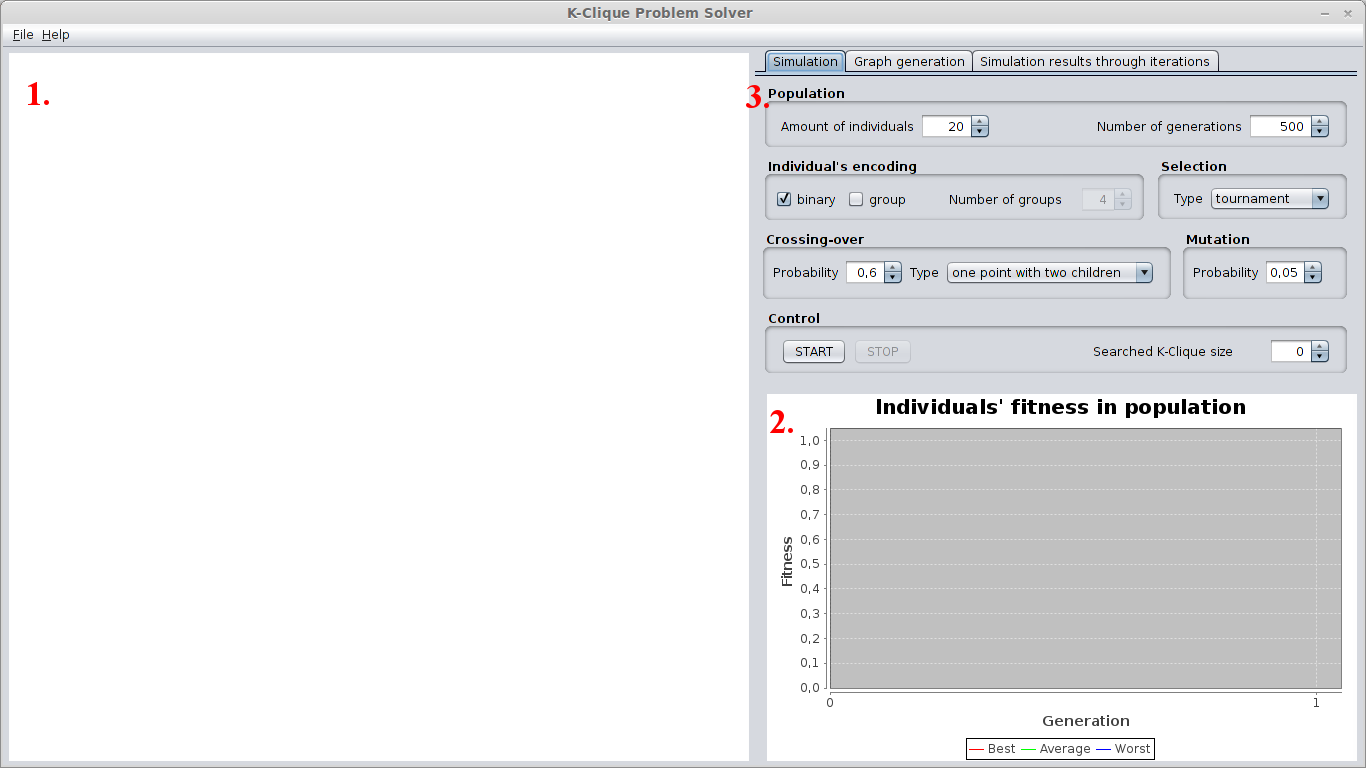
\includegraphics[width=16cm]{interfejs}

Program składa się~z~trzech głównych sekcji:
\begin{enumerate}[noitemsep]
 \item wizualizacji grafu;
 \item wykresu;
 \item panelu sterowania.
\end{enumerate}

Pierwsze dwie zostaną bliżej pokazane w~kolejnych podpunktach. Panel sterowania składa się~z~trzech podpaneli (odpowiednie zakładki):


\includegraphics[width=14cm]{zakladki}

Jak wskazują nazwy służą one kolejno do:
\begin{itemize}[noitemsep]
 \item zarządzania symulacją - ustalanie parametrów, start/stop;
 \item generowania grafu - opcje generowania grafu o~zadanej liczbie wierzchołków i~krawędzi, a~także zawierającego klikę o~żądanym rozmiarze,
 wczytywania/zapisywania grafu z/do~pliku oraz rysowania grafu;
 \item przeglądania wyników symulacji, czyli wyświetlaniu najlepszego rozwiązania dla~zadanej iteracji.
\end{itemize}

\section{Zmienne parametry algorytmu}
\label{sec:params}
Oprócz wejściowego grafu użytkownik ma~możliwość ustalić:
\begin{itemize}[noitemsep]
 \item liczebność populacji - im~większa, tym~wolniej będzie przebiegać symulacja, jednak uzyskane wyniki powinny być~lepsze;
 \item maksymalną liczbę iteracji - jeżeli algorytm nie znajdzie kliki o~zadanym rozmiarze wcześniej, zakończy działanie po~ustalonej tutaj liczbie iteracji;
 \item sposób kodowania - użytkownik ma~do~wyboru kodowanie binarne i~grupowe, oba opisane wcześniej, w~drugim przypadku możliwe jest również ustalenie 
początkowej ilości grup;
 \item typ selekcji - trzy wymienione wyżej możliwości przeprowadzania procesu selekcji;
 \item prawdopodobieństwo krzyżowania;
 \item sposób krzyżowania - sześć różnych metod krzyżowania;
 \item prawdopodobieństwo mutacji;
 \item rozmiar szukanej kliki.
\end{itemize}

\section{Przebieg pojedynczej iteracji}
\label{sec:singleLifeCycle}
Każda iteracja algorytmu składa się~z:
\begin{itemize}[noitemsep]
 \item selekcji, czyli wyboru grupy rodziców (z~możliwymi duplikatami), z~których powstanie nowe pokolenie dzieci;
 \item krzyżowania, czyli utworzenia nowej populacji (dzieci) z~wybranych wcześniej osobników (rodziców) przy pomocy wybranego typu krzyżowania (stosowanego z~
 uwzględnieniem prawdopodobieństwa krzyżowania);
 \item mutacji genotypu niektórych osobników zgodnie z~zadanym prawdopodobieństwem;
 \item usunięcia najgorszych osobników;
 \item poprawienia liczebności populacji, czyli operacji mającej na celu utrzymanie stałej ilości osobników w~populacji;
 (polega na~uzupełnieniu populacji nowo utworzonymi (losowymi) osobnikami, jeśli rozmiar populacji był~zbyt~mały, lub~na~usunięciu
 najgorszych jednostek w~przeciwnym wypadku);
 \item sprawdzenia warunku stopu.
\end{itemize}
Dodatkowo, w~kodowaniu grupowym w~odpowiednich iteracjach następuje usunięcie najsłabszej grupy (podgrafu o~najniższej wartości funkcji przystosowania).

\section{Wykres przystosowania}
\label{sec:chart}
\begin{figure}[ht]
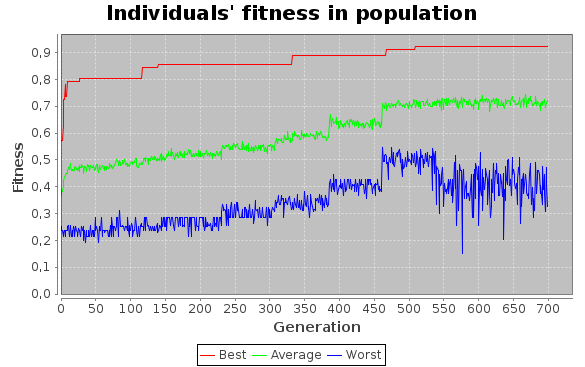
\includegraphics[width=16cm]{chart} 
\end{figure}
Wykres jest rysowany równolegle z~przebiegiem algorytmu. Przedstawia wartości funkcji przystosowania najlepszego (czerwony) i~najgorszego
(niebieski) osobnika w populacji, oraz wartość średnią funkcji przystosowania wszystkich osobników (zielony) w~każdym kolejnym pokoleniu.
\vspace*{100mm}

\section{Wizualizacja grafu}
\label{sec:visualization}

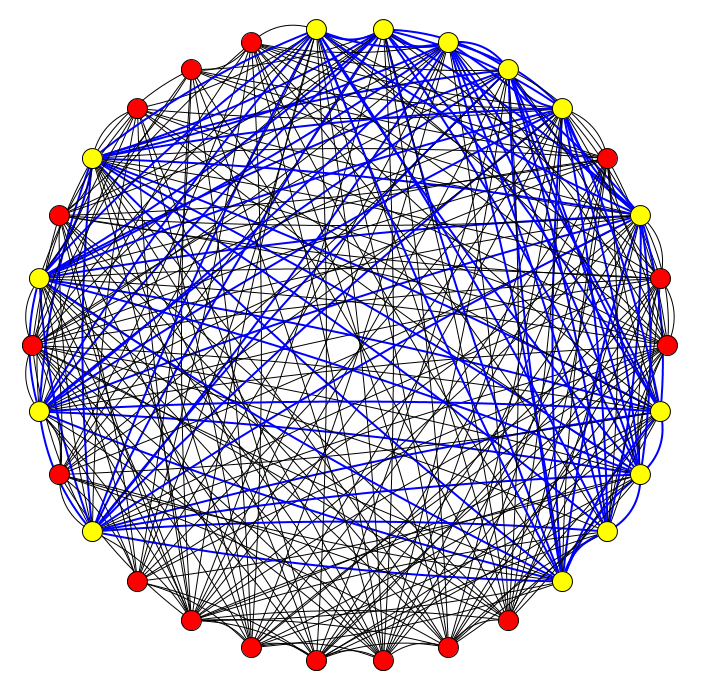
\includegraphics[width=16cm]{graf}

Wizualizowany graf jest aktualizowany równolegle z~przebiegiem algorytmu, co~5~iteracji. Rozwiązanie - najlepszy osobnik w~populacji - 
zostało wyróżnione żółtymi wierzchołkami i~niebieskimi, pogrubionymi krawędziami.

Aplikacja pozwala wybrać sposób prezentowania grafu, jednak zalecanym jest przedstawiony powyżej (o~nazwie~\textit{circle}).

\chapter{Źródła} 
\label{cha:sources}

Podczas opracowywania rozwiązania problemu korzystaliśmy z:
\begin{itemize}[noitemsep]
 \item dr inż. Lidia Dutkiewicz, wykład \textit{Algorytmy ewolucyjne};
  \item dr inż. Piotr Urbanek, wykład \textit{Algorytmy genetyczne};
 \item Michał Bereta, Paweł Jarosz \textit{Algorytmy genetyczne};
 \item James A. Foster, Terry Soule \textit{Using Genetic Algorithms to Find Maximum Cliques};
 \item Harsh Bhasin, Rohan Mahajan \textit{Genetic Algorithms Based Solution To
Maximum Clique Problem};
\item \textit{http://en.wikipedia.org/wiki/Genetic\_algorithm};
 \item \textit{http://pl.wikipedia.org/wiki/Problem\_kliki}; % ze znacznikami \url to zle wyglada :(
 \item \textit{http://pl.wikipedia.org/wiki/Problem\_NP-zupelny};
 \item \textit{http://pl.wikipedia.org/wiki/Algorytm\_genetyczny};
 \item \textit{http://www.k0pper.republika.pl/geny.htm}.
\end{itemize}



%% tu nie moje.
%\include{rozdzial1}
%\include{rozdzial2}



% itd.
% \appendix
% \include{dodatekA}
% \include{dodatekB}
% itd.

%\bibliographystyle{alpha}
%\bibliography{bibliografia}
%\begin{thebibliography}{1}
%
%\bibitem{Dil00}
%A.~Diller.
%\newblock {\em LaTeX wiersz po wierszu}.
%\newblock Wydawnictwo Helion, Gliwice, 2000.
%
%\bibitem{Lam92}
%L.~Lamport.
%\newblock {\em LaTeX system przygotowywania dokumentów}.
%\newblock Wydawnictwo Ariel, Krakow, 1992.
%
%\bibitem{Alvis2011}
%M.~Szpyrka.
%\newblock {\em {On Line Alvis Manual}}.
%\newblock AGH University of Science and Technology, 2011.cccccc
%\newblock \\\texttt{http://fm.ia.agh.edu.pl/alvis:manual}.
%
%\end{thebibliography}

\end{document}